\documentclass[a4paper,11pt,twoside,abstraction,titlepage]{article}

\usepackage{verbatim}
\usepackage{latexsym}
\usepackage{exscale}
\usepackage{makeidx}
\usepackage{textcomp}
\usepackage{amsmath}
\usepackage{amsthm}
\usepackage{amssymb}
\usepackage{mathrsfs}
\usepackage{graphicx}
\usepackage{caption}
\usepackage{enumerate}
\usepackage{url}
\usepackage{booktabs}
\usepackage{wrapfig}
\usepackage{framed}




\title{\Large \bf Implementation of Imputation Algorithm}
\author{Michelle Parker}

\linespread{1.03}

\begin{document}

\maketitle

\begin{abstract}
Accurate and fast imputation of genotype data is an increasing requirement as a surge of low coverage sequence data is being produced.  This report describes the techniques and algorithms used in the imputation software BEAGLE 2.1.  A Python implementation emulating the BEAGLE algorithms has been tested to show similar accuracy on the same number of samples and markers but with a very slow run time.  ?? conclusion??
\end{abstract}

\clearpage
\setcounter{tocdepth}{2}
\tableofcontents

 
\newpage

\section{Introduction}
The statistical definition of imputation is "a procedure for entering a value for a specific data item where the response is missing or unusable" \cite{unece}. In genetics, imputation refers to the process of inferring genotypes that are either missing, have a low quality score or are not directly assayed in sampled individuals.  This technique is used increasingly in genome-wide association and whole genome sequencing studies. 

Imputation has several uses: to boost power in a study by inferring erroneous, low confidence or sporadic missing data; to refine genotype probabilities; and to infer untyped data by using a reference panel containing a larger set of genetic markers.

In genome-wide association studies (GWAS), a number of genetic variants, usually single-nucleotide polymorphisms (SNPs), are assayed in groups of individuals with and without the disease of interest.  The selection of genetic variants used in the study are often genotyped using DNA microarrays; distinct types of microarray are composed of different selections of genetic variants across the genome.

Multi-marker association analysis, used in GWAS, identifies markers that are independently associated to the disease of interest.  Imputing sporadic missing data can make it easier to interpret the results of these analyses and can also boost power.  There may also be a number of genotype calling errors due low confidence data.  Imputation can be used to correct these errors which may help to control false-positive associations. \cite{review2009}.

A reference panel is a collection of samples genotyped at a dense set of markers across the genome.  These known haplotypes can be used to impute genetic variants that are not included on the SNP array used in the study.  This increases the number of SNPs that can be tested for association and advances fine-mapping studies where the location of the causal variant is identified. This technique can also be used in meta-analysis, where two or more studies conducted on different platforms are combined.  Stronger associations may be found with untyped SNPs than those that are genotyped even if the untyped SNP is poorly tagged, because imputation algorithms estimate haplotypes taking into account multiple markers surrounding the missing genotype \cite{review2010}.

The process of imputation is illustrated in Figure 1. Imputation is based on the identification of stretches of haplotypes which are shared between individuals.  These regions are known as being identical-by-descent (IBD) and would have originated from identical copies of the same ancestral allele.  Regions of IBD are much longer in closely related individuals than in unrelated individuals. In both related and unrelated samples, imputed haplotypes are modelled as mosaics of haplotypes in the reference panel.  When there is uncertainty over which haplotype is IBD, many imputation programs take this into account and summarize the information probabilistically.  Genotype likelihoods give a more accurate representation of the data and can often lead to more significant results when used in downstream analysis \cite{review2010}.

\begin{figure}[tp]
\begin{center}
\centerline{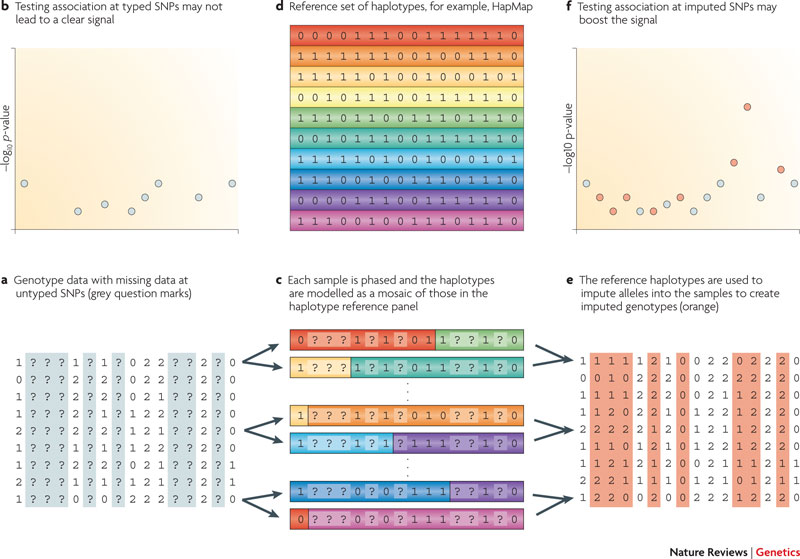
\includegraphics[scale=0.58]{reviewimage}}
\vspace{20pt}
\caption{This figure illustrates imputation of untyped SNPs in a sample of unrelated individuals using a reference panel \cite{review2010}.
\newline
Samples in the study are genotyped at a small number of sites using a microarray ({\bf a}). A reference panel ({\bf d}) of denser SNPs is used to infer the SNPs that have not been directly genotyped in the samples ({\bf c}).  In this process the samples are phased and the untyped SNPs are imputed ({\bf e}).
\newline
Testing association on just the SNPs which are directly assayed ({\bf a}) may not lead to a significant result ({\bf b}) but testing on all SNPs after imputation ({\bf e}), stronger associations on inferred SNPs may be found ({\bf f}).}
\end{center}
\vspace{-10pt}
\end{figure}

In low coverage whole genome sequencing, such as in the 1000 Genomes Project \cite{1000genomes}, imputation is used to assist genotype likelihood estimation and calling.  Relatively small amounts of sequence data across many individuals is combined to accurately estimate the genotypes for each sample.  In other words, the imputation algorithms use the sample data itself as its own reference panel.  Imputation can also be extended to include non-SNP variation such as copy number variation, classical human leukocyte antigen alleles, and short insertions and deletions (indels) \cite{review2010}.

There are many different methods for imputation based on different statistical models, but imputation algorithms can be divided into two main categories: those which take into account all observed genotypes during its computation of a single sample (IMPUTE, MACH, fastPHASE/BIMBAM), and those which only look at a window of markers either side of the missing genotype (BEAGLE, PLINK) \cite{review2009}.  Using all observed genotypes is computationally expensive but in many cases can achieve a more accurate result.  Factors which affect imputation accuracy include the size and choice of reference panel; the difference in genetic diversity between the study population and the reference panel; use of tagging methods for SNP array design.  In almost all cases, the more samples in the reference panel, the more accurate the imputation.  The algorithm implemented in this report uses a probabalistic graphical model and is described in the BEAGLE paper \cite{beagle3}.


\newpage
\section{Methods}
The BEAGLE algorithm has a similar structure to the expectation maximization (EM) algorithm \cite{EMalgorithm}.  An initial estimate of haplotype phase is obtained for each individual and then at each iteration, the model is fit and an improved estimate of haplotype phase per individual is sampled.  The final output haplotypes are obtained by calculating the most likely haplotype pairs per individual conditional on the model in the final iteration.

The process can therefore be split into 3 sections: model building, where a probabilistic graphical model is used to implicitely cluster haplotypes; sampling, where haplotypes are re-estimated and used as input into the next model build; and a maximization step, where the most likely haplotypes are computed based on the current model.

The haplotype-clustering model which is built defines a Hidden Markov Model (HMM) where a modified forward-backward algorithm can be used for the sampling step and the Viterbi algorithm can be used for the maximization.  The BEAGLE recommendation is to run 10 iterations of the model building and sampling steps before carrying out the Viterbi algorithm.


\subsection{Model Building}
The model is represented as a directed acyclic graph.  Assuming no missing alleles and a collection of samples genotyped at $M$ markers, the directed graph has the following properties:

\vspace{-5pt}
\begin{enumerate}
\itemsep0pt
\item The graph is levelled with $M+1$ levels. Each node of the graph is a member of a level that corresponds to the position in the sequence of markers.
\item At level $1$, there is one root node which has no incoming edges.  At level $M+1$ there is one terminal node which has no outgoing edges.
\item All incoming edges to a node at level $m$ have a parent node at level $m-1$.  All outgoing edges from the node at level $m$ have a child node at level $m+1$.
\item Each edge at level $m$ is marked by a single allele $a$.  Two edges originating from the same parent node can not be labelled with the same allele.
\item There exists a path from the root node to the terminal node for each haplotype in the samples such that the $m$th allele of the haplotype is the label of the $m$th edge of the path.
\end{enumerate}


\begin{figure}[htp]
\centering
\begin{tabular}{lc}
\toprule
Haplotype & Count \\
\midrule
1111 & 21\\ 
1112 &  79\\
1122 & 95\\
1221 & 116 \\
2111 & 25\\
2112 & 112\\
2122 & 152\\
\bottomrule 
\end{tabular}
\vspace{5pt}
\caption{Summary genotype data from 300 individuals}

\vspace{-5pt}
\end{figure}


\noindent The model building algorithm will be exemplified using data in Figure 2.   The algorithm begins by inserting genotype data from each indivudal into the graph.  The data is processed a marker at a time.  If the phase is not known, the data is randomly phased.  If the marker is missing, the marker is randomly imputed based on population allele frequencies at that marker.  Each path from the root node to the terminal node represents a single haplotype and the results inserting data from Figure 2 into the model format is shown in Figure 3.

\begin{figure}[htp!]
\vspace{10pt}
\begin{center}
\centerline{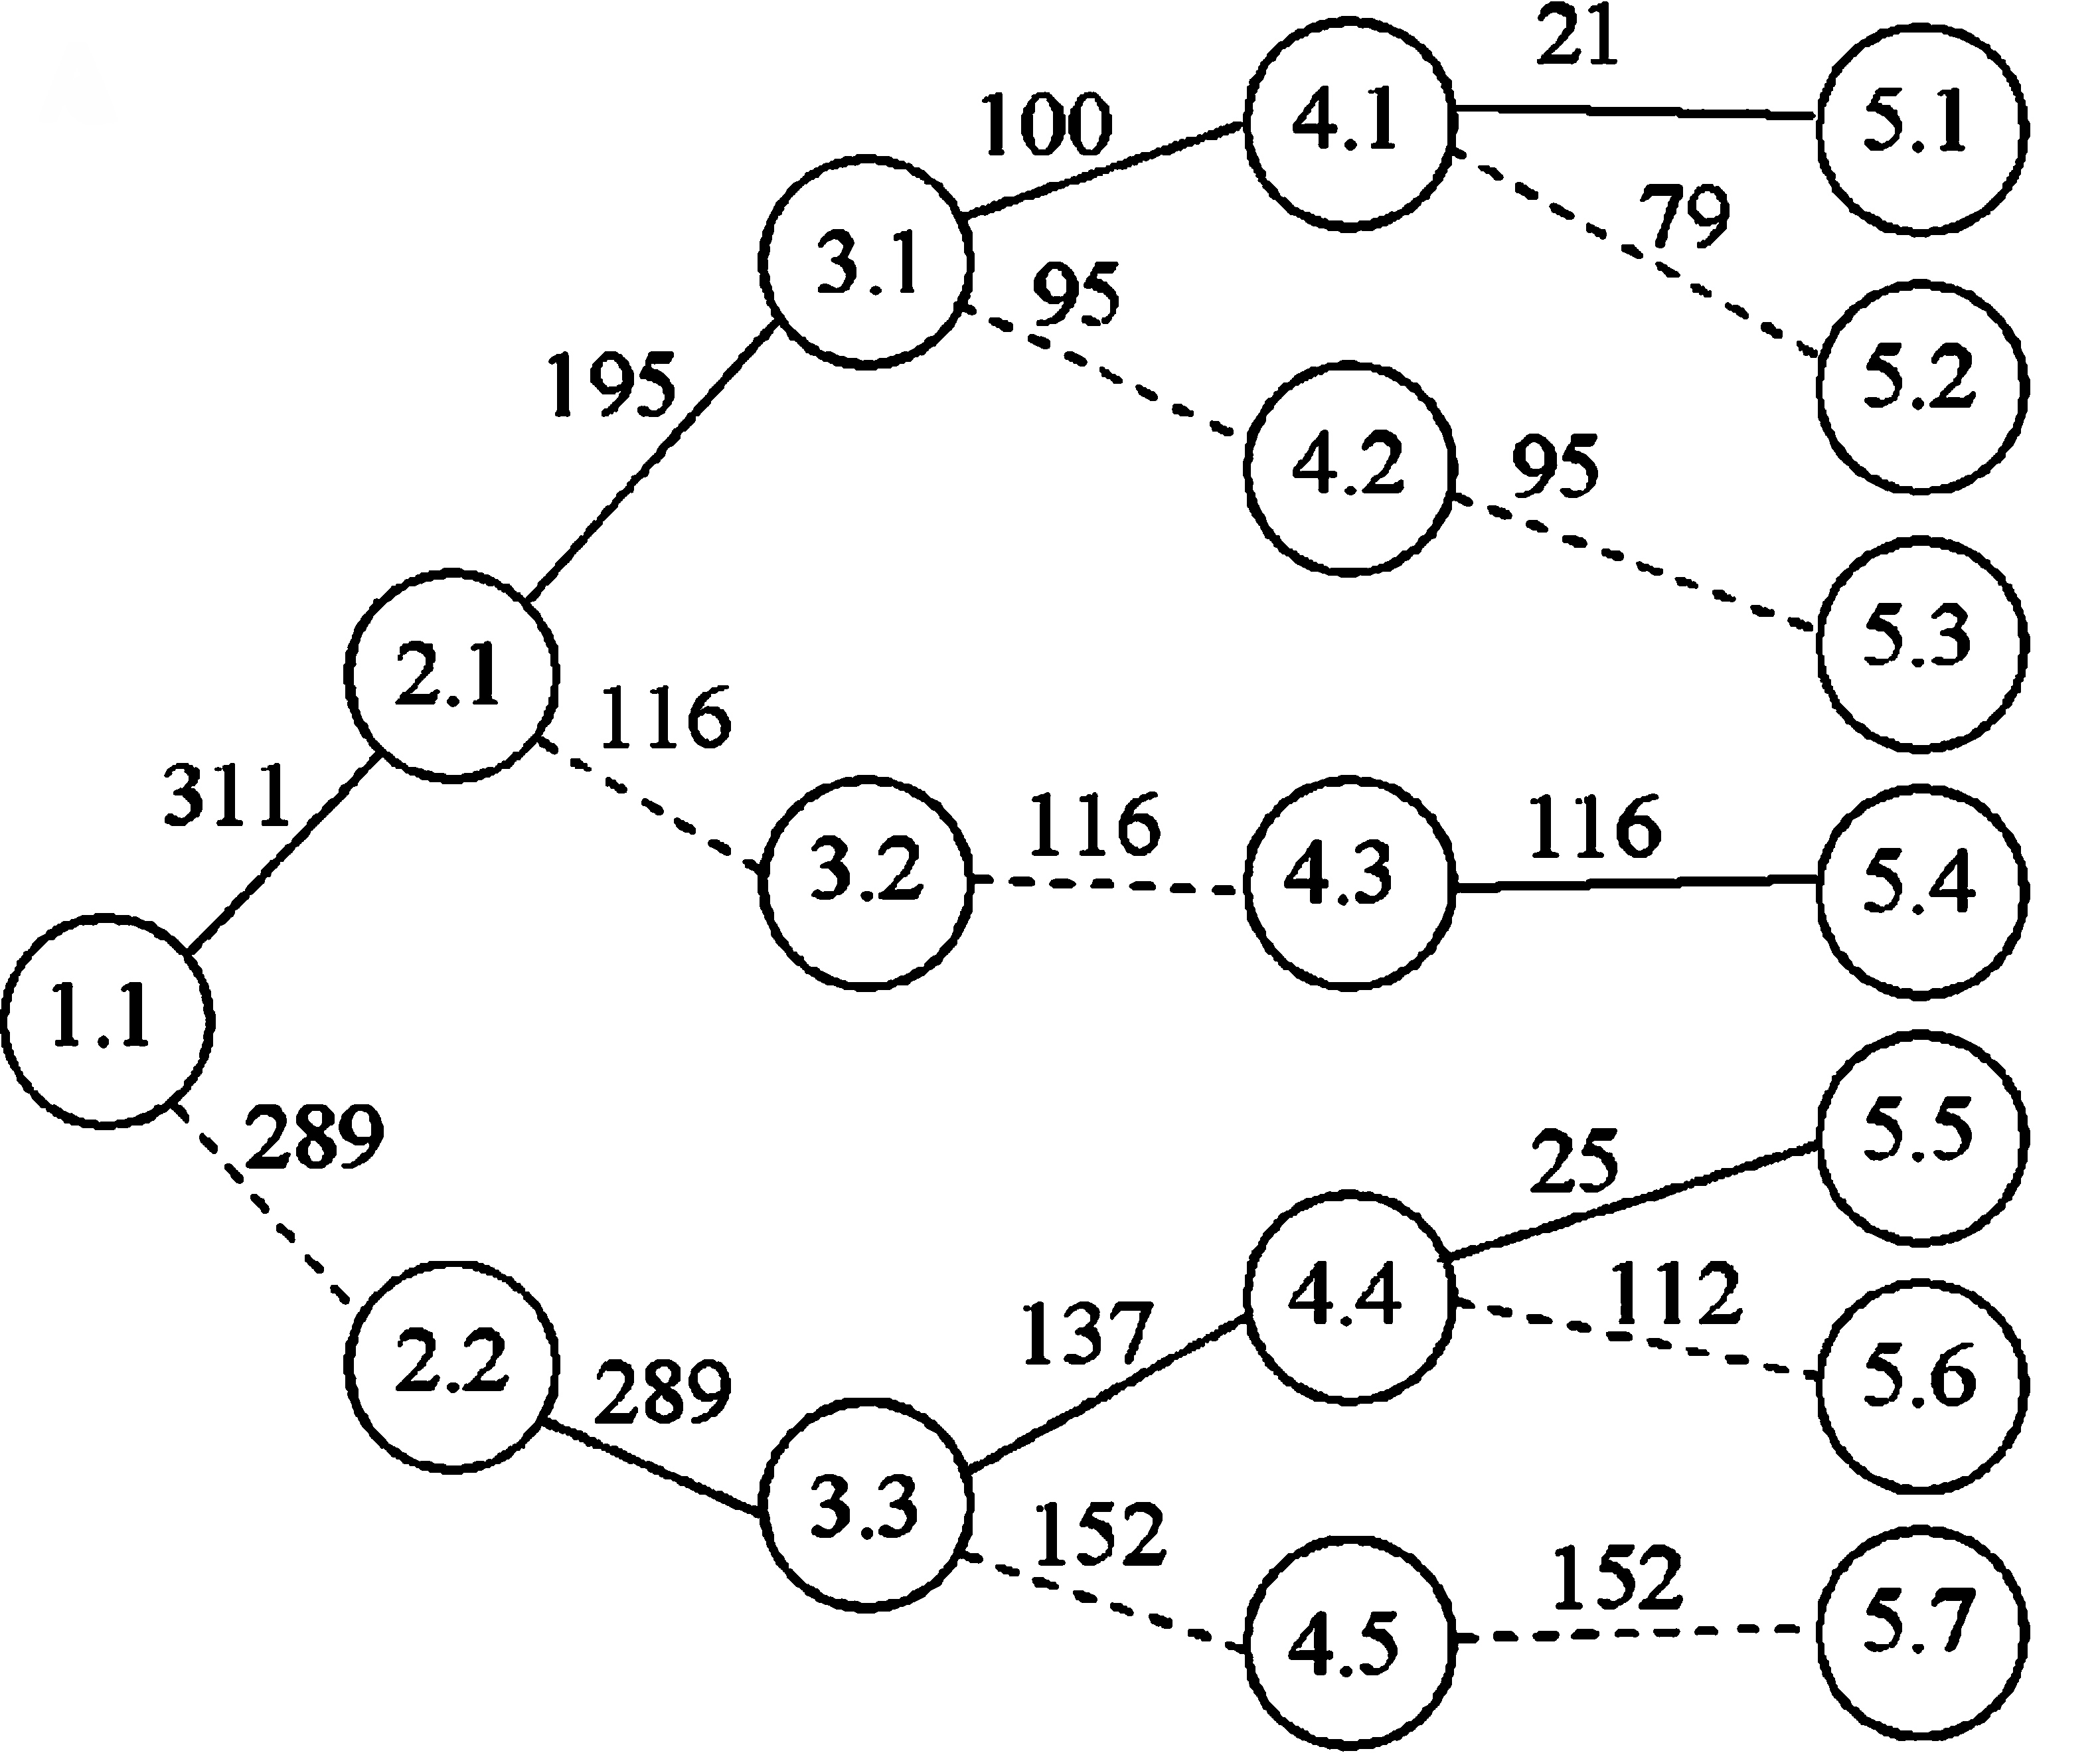
\includegraphics[scale=0.08]{fig3}}
\vspace{2pt}
\caption{Tree constructed using summary genotype data in Figure 2. Circles are nodes and lines are edges. A solid edge represents the allele 1 and dashed edge represents the allele 2. Numbers above the edges represent haplotype counts.  This graph is directional from left to right. \cite{beagle1}}

\end{center}
\vspace{-25pt}
\end{figure}


After this tree has been created, it then needs to be compressed into the graph format described at the beginning of this section.  The tree is condensed into a graph format by merging pairs of nodes on each level which are sufficiently similar.  The algorithm iterates through each level at a time and merges all pairs of nodes where transition probabilities of all downstream nodes pass a certain threshold.  All nodes at the final level are merged to create the single terminal node that represents the cluster of all haplotypes after being processed by the model.

The similarity score between nodes $x$ and $y$ on level $m-1$ is calculated as follows.  Let $n_x$ be the haplotype count at node $x$ and $n_y$ be the haplotype count at node $y$.  For allele $a_m$ at level $m$, let $n_x(a_m)$ be the count of haplotypes which pass through node $x$ and then begin with marker $a$.  Similarly, let $n_y(a_m)$ be the count of haplotypes which pass through node y and then begin with marker $a$.  Continuing, $n_x(a_m,a_{m+1})$ and $n_y(a_m,a_{m+1})$ are haplotype counts which pass through nodes $x$ and $y$ respectively and follow with the sequence of alleles $a_m,a_{m+1}$.  The observed conditional probability difference diff$_{xy}$ between node $x$ and $y$ for given sequence of alleles $a_m,a_{m+1},...,a_{m+k}$ is
\begin{equation*}
\mbox{diff}_{xy} = \left|\frac{n_x(a_m,a_{m+1},...,a_{m+k})}{n_x} - \frac{n_y(a_m,a_{m+1},...,a_{m+k})}{n_y}\right|
\end{equation*}


\noindent The similarity score for nodes $x$ and $y$ is the maximum diff$_{xy}$ over $k=0, 1, 2,..., M-m$ and all possible $a_m,a_{m+1},...,a_{m+k}$.

The algorithm iterates through each level in the graph and calculates the similarity score between all pairs of nodes and merges the pair that have the lowest similarity score below the corresponding threshold.  The threshold between two nodes $x$ and $y$ is defined as $(n_x^{-1} + n_y^{-1})^{\frac{1}{2}}$.  All nodes are merged into one at the final level.

\begin{figure}[htp!]

\begin{center}
\centerline{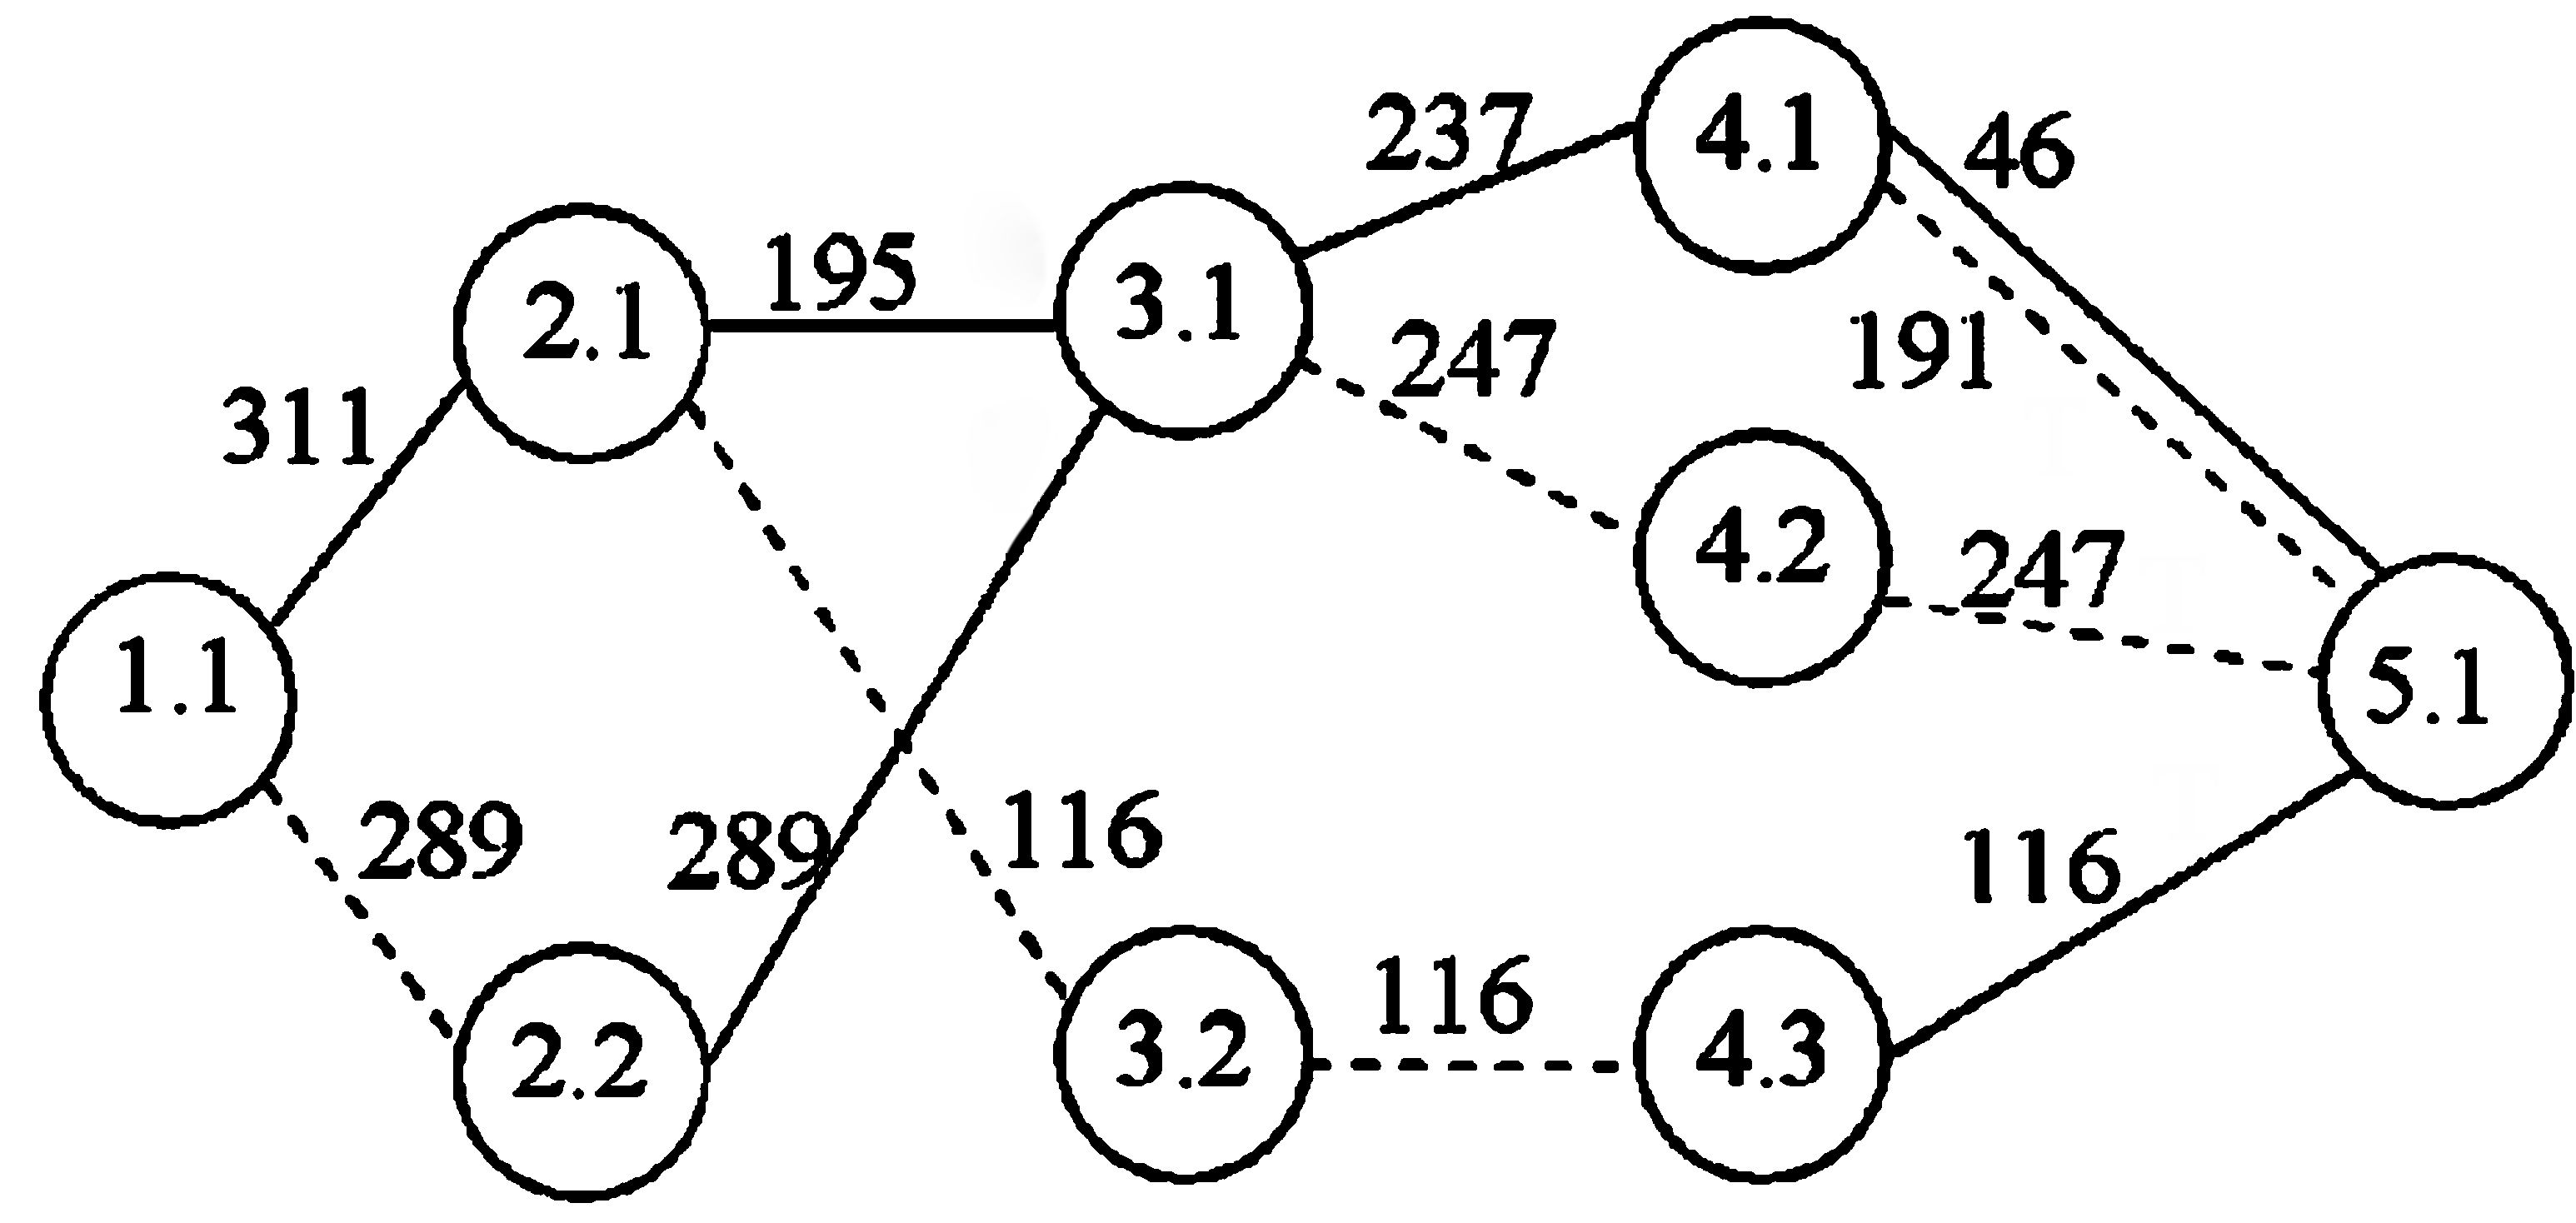
\includegraphics[scale=0.08]{fig4}}
\caption{Merged graph.  Nodes 3.1 and 3.3 in Figure 2 have merged into node 3.1 and all nodes in the final level have been merged into node 5.1 \cite{beagle1}.}

\end{center}
\vspace{-20pt}
\end{figure}

\noindent Consider Figure 3 as an example.   The similarity threshold for nodes 2.1 and 2.2 is 
\vspace{-5pt}
\begin{equation*}
\left(\frac{1}{311}+\frac{1}{289}\right)^{\frac{1}{2}} = 0.082
\end{equation*}
Beginning the calculation of the similarity score of these two nodes, first calculate diff$_{2.1,2.2}$ for allele $a_2=1$.
\begin{equation*}
\mbox{diff}_{xy} = \left|\frac{195}{311}-\frac{289}{289}\right| = 0.373
\end{equation*}
The similarity score is the maximum score of all diff$_{xy}$ and is therefore at least 0.373.  This exceeds the cutoff at 0.082 and therefore these two nodes will not be merged.

\vspace{8pt}
\noindent At level 3, similarity scores for all pairs are calculated.  The threshold for nodes 3.1/3.2 is 
\vspace{-5pt}
\begin{equation*}
\left(\frac{1}{195}+\frac{1}{116}\right)^{\frac{1}{2}} = 0.117
\end{equation*}
For $a_3=1$,
\begin{equation*}
\mbox{diff}_{xy} = \left|\frac{100}{195}-\frac{0}{116}\right| = 0.513
\end{equation*}
which does exceeds the threshold and therefore nodes can not be merged.

\vspace{8pt}
\noindent The threshold for nodes 3.2/3.3 is
\vspace{-5pt}
\begin{equation*}
\left(\frac{1}{116}+\frac{1}{289}\right)^{\frac{1}{2}} = 0.110
\end{equation*}
For $a_3=1$,
\begin{equation*}
\mbox{diff}_{xy} = \left|\frac{0}{116}-\frac{137}{289}\right| = 0.474
\end{equation*}
which exceeds the threshold and therefore nodes can not be merged.

\vspace{8pt}
\noindent The threshold for nodes 3.1/3.3 is
\vspace{-5pt}
\begin{equation*}
\left(\frac{1}{195}+\frac{1}{289}\right)^{\frac{1}{2}} = 0.093
\end{equation*}
diff$_{xy}$ is calculated for every suffix combination.
\vspace{8pt}

\noindent For $a_3=1$,
\begin{equation*}
\mbox{diff}_{xy} =\left|\frac{100}{195}-\frac{137}{289}\right| = 0.039 
\end{equation*}
For $a_3=2$,
\begin{equation*}
\mbox{diff}_{xy} =\left|\frac{95}{195}-\frac{152}{289}\right| = 0.039
\end{equation*}
For $a_3=1, a_4=1$,
\begin{equation*}
\mbox{diff}_{xy} =\left|\frac{21}{195}-\frac{25}{289}\right| = 0.021
\end{equation*}
For $a_3=1, a_4=2$,
\begin{equation*}
\mbox{diff}_{xy} =\left|\frac{79}{195}-\frac{11}{289}\right| = 0.018
\end{equation*}
For $a_3=2, a_4=2$,
\begin{equation*}
\mbox{diff}_{xy} =\left|\frac{95}{195}-\frac{152}{289}\right| = 0.039
\end{equation*}
\vspace{1pt}

\noindent Thus the similarity score for nodes 3.1/3.3 is the maximum of all diff$_{xy}$.
\begin{equation*}
max(0.039, 0.039, 0.021, 0.018, 0.039) = 0.039
\end{equation*}
The similarity score is less than the threshold value and therefore these two nodes are able to be merged.

This level contains only 3 nodes (3.1, 3.2, 3.3) and from the 3 combinations of pairs, only the pair (3.1, 3.3) has a score below the corresponding threshold value for the pair of nodes.  Therefore in this example, 3.1/3.3 are the only pair which can be merged at this stage.  Merging these two nodes involves the summation of all downstream haplotype paths.  All incoming edges to node 3.3 are moved to node 3.1.  All values of downstream paths from 3.3 are added to the values of 3.1.  After this process the node 3.3 is deleted, leaving only two nodes on that level (3.1, 3.2).  The similarity score is re-calculated for all remaining nodes and again the lowest scoring pair of nodes which pass the corresponding threshold are merged.  This repeats until no merges can happen.  In this example, the similarity score is recalculated for nodes 3.1/3.2.

\vspace{10pt}

\noindent The threshold for nodes 3.1/3.2 is
\vspace{-5pt}
\begin{equation*}
\left(\frac{1}{484}+\frac{1}{116}\right)^{\frac{1}{2}} = 0.103
\end{equation*}
For $a_3=1$,
\begin{equation*}
\mbox{diff}_{xy} = \left|\frac{237}{484}-\frac{0}{116}\right| = 0.490
\end{equation*}
which exceeds the threshold and therefore no nodes can be merged again at this level.
\vspace{8pt}

\noindent No nodes are merged on level 4 and all nodes are merged on the final level.  The resultant graph is shown in Figure 4. \cite{beagle1}

The advantage of this graph is that it provides a parsimonious model which is able to adapt to the local structure of the data.  Linkage disequilibrium (LD) is the non-random association of two or more alleles.  This means the occurence of combinations of alleles which occur more often or less often than would be expected by random formation of haplotypes based on allele frequencies.  This occurs because the closer two loci are on a chromosome, the more likely they are to be inherited from a single ancestrial allele; ie. correlation between markers decreases with distance.

The level of LD can be influenced by a number of factors (selection, rate of recombination, rate of mutation, non-random mating) and is important in accurately predicting phase and imputing missing alleles.  The graph implicitely models localized changes in linkage disequilibrium by dynamically clustering different selections of haplotypes at different positions.  The number of clusters at each marker is also influenced by the data. \cite{LDwiki}

An edge represents a cluster of haplotypes whose path from the initial node to the terminal node passes through the edge.  These haplotypes tend to have similar patterns of alleles at markers surrounding the edge and therefore each edge defines a localized haplotype cluster.  In regions of low LD, fewer merges and more clusters are expected, and in regions of high LD more merges and fewer haplotype clusters are expected. \cite{beagle2}



\subsection{Induced Hidden Markov Model (HMM)}
Haplotypes are grouped together at position $a$ if they have simliar downstream transition probabilities.  This means that haplotype clusters at position $a$ are defined by the Markov property: the sequence of alleles at markers $a, a-1, a-2, ...$ are independent of the sequence of alleles at markers $a+1, a+2, ...$.  This means the localized hapotype cluster model can be used to define an HMM where the states are the edges and the emitted symbol for each state is the allele that labels the edge.

\begin{figure}[htp!]
\begin{center}
\centerline{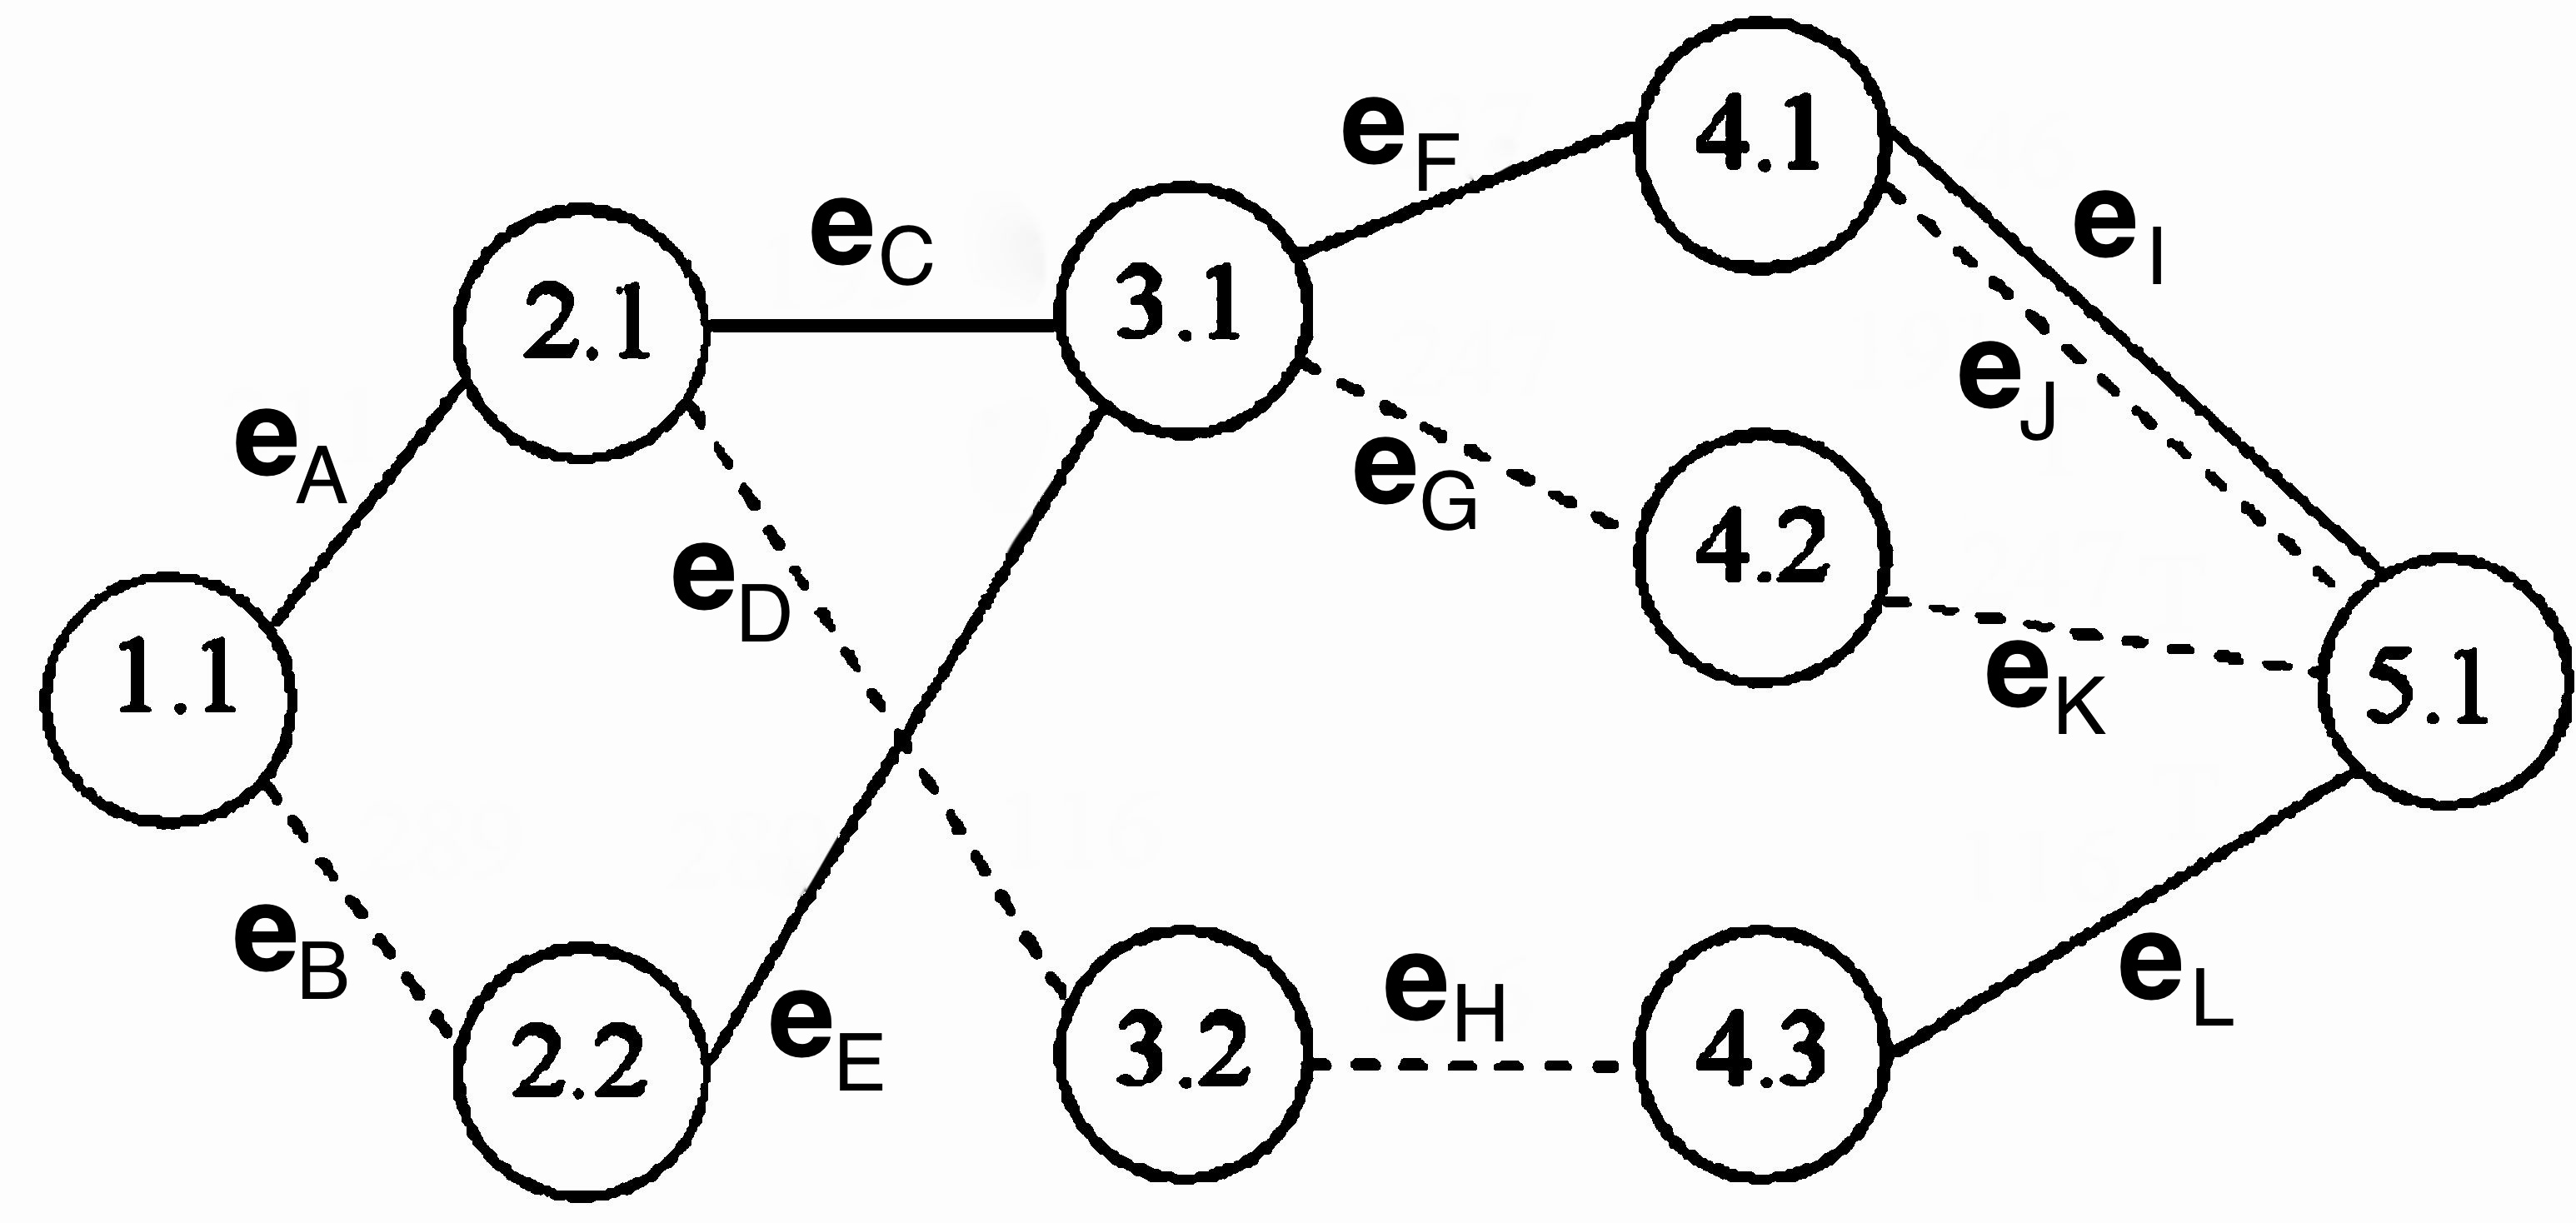
\includegraphics[scale=0.08]{fig5}}
\caption{Copy of merged graph in Figure 4 with edges labelled. \cite{beagle1}.}
\end{center}
\vspace{-20pt}
\end{figure}

\noindent Let $n(e)$ define the haplotype count at edge $e$ and $n_p(e)$ define the haplotype count at the parent node of edge $e$.  Each state (edge) emits with probability 1 the allele that labels the edge.  Therefore each state uniquely determines the observed allele but the observed marker does not determine the state, as at a particular level there may be many edges labelled with the same allele.

\noindent The initial state probabilities are determind by the edge counts.  
\begin{equation*}
P(e) = 
\begin{cases}
\frac{n(e)}{n_p(e)} & \mbox{if parent node of $e$ is the root node} \\
0  & \mbox{otherwise}
\end{cases}
\end{equation*}
The transition probabilities are defined as follows.
\begin{equation*}
P(e_1|e_2) = 
\begin{cases}
\frac{n(e_1)}{n_p(e_1)} & \mbox{if parent node of $e_1$ is the child node of edge $e_2$} \\
0  & \mbox{otherwise}
\end{cases}
\end{equation*}
This has described a haploid HMM but a diploid HMM is needed because genotype data is used.  The diploid HMM is created from ordered pairs of edges in each level of the graph.  The level of the parent node of an edge defines the level of the edge therefore in a graph with $M+1$ levels, the states of the HMM (edges) can be partioned into $M$ classes $L_m$, where $m=1,2,...,M$.  The edges of the graph in Figure 5 are partioned in the following way.
\vspace{-10pt}
\begin{align*}
L_1 &= \{e_{A}, e_{B}\} \\
L_2 &= \{e_{C}, e_{D}, e_{E}\}\\
L_3 &= \{e_{F}, e_{G}, e_{H}\} \\
L_4 &= \{e_{I}, e_{J}, e_{K}, e_{L}\}
\end{align*}

\noindent The state space for the diploid HMM is the union over $m$ of ($L_m \times L_m$).  Each state (ordered pair of edges) emits with probability 1 the unordered alleles that label the edges.  Therefore the diploid HMM emits an unordered genotype.  The initial probabilities and the transition probabilities are the product of the corresponding haploid probabilities.

\vspace{10pt}
\noindent The initial state probabilities:
\begin{equation*}
P(e_1,e_2) = P(e_1)P(e_2)
\end{equation*}
Transition state probabilties:
\begin{equation*}
P[(e_1,e_2)|(e_3,e_4)] = P(e_1|e_3)P(e_2|e_4)
\end{equation*}

\noindent The Hary-Weinberg principle is assumed. \cite{beagle2}

\newpage
\subsection{Forwards Algorithm and Backwards Sampling}
A modified forwards algorithm is used to sample genotypes from the diploid model conditional on the observed data.  Let $g_m$ be the observed unordered genotype at marker $m$ for an individual.  Let the state $s_m = (e_1, e_2)$ be an ordered pair of edges in $L_m \times L_m$.

In a graph with $M+1$ levels, an individual's genotypes is $\{g_1, g_2, ... , g_M\}$.  The forward variable is defined as 
\begin{equation*}
\alpha_m(s_m) = P(g_1,g_2,...,g_m,s_m)
\end{equation*}

\noindent In other words, the forward variable is the probability of the observed unordered genotypes up to marker $m$ and the ordered state $s_m$ at marker $m$ given the current model.  This can be solved inductively as follows.

\vspace{10pt}
\noindent 1. Initiation
\begin{equation*}
\alpha_1(s_1) = P(g_1, s_1) = P(s_1) P(g_1|s_1)
\end{equation*}

\begin{framed}
\begin{tabular}{lll}
\hspace{-20pt} $P(s_1)$ & : & \hspace{-5pt}Probability the ordered state is $s_1$ at marker 1 (initial)\\
\hspace{-20pt} $P(g_1|s_1)$ & :& \hspace{-5pt}Probability $g_1$ is observed given the state $s_1$ (emission)
\end{tabular}
\end{framed}


\vspace{10pt}
\noindent 2. Induction
\begin{eqnarray*}
\alpha_{m+1}(s_{m+1}) &=& P(g_1,g_2,...,g_{m+1},s_{m+1})     \\
&=& \sum\limits_{s_m} P(g_1,g_2,...,g_m, g_{m+1}, s_m, s_{m+1}) \\
&=&  \sum\limits_{s_m} P(g_1,g_2,...,g_m,, s_m) P(g_{m+1}|s_{m+1}) P(s_{m+1}|s_m) \\
&=& P(g_{m+1}|s_{m+1}) \sum\limits_{s_m} \alpha_m(s_m) P(s_{m+1}|s_m) 
\end{eqnarray*}

\begin{framed}
\begin{tabular}{lll}
\hspace{-20pt} $P(g_{m+1}|s_{m+1})$ &:& \hspace{-5pt} Probability $g_{m+1}$ is observed given the state \\
&& $s_{m+1}$ (emission) \\
\hspace{-20pt}  $\sum\limits_{s_m} \alpha_m(s_m)$ &:& \hspace{-5pt} Sum of probabilities of all branches of the tree \vspace{-7pt} \\ 
&& where state is $s_m$ at level $m$ \\
\hspace{-20pt} $P(s_{m+1}|s_m)$ &:& Probability state is $s_{m+1}$ at level $m+1$ given the \\
&& state is $s_m$ at level $m$ (transition)
\end{tabular}
\end{framed}

\noindent Forward probabilities are calculated for every possible combination of ordered edges at each level (states) using the observed genotype sequence for an individual ${g_1, g_2, ..., g_M}$.  The role of imputation is to infer the missing alleles in an individual's genotype.  At a specific marker position, if both alleles of $g_m$ are missing, then the emission probability $P(g_m|s_m) = 1$ for every state.  If one allele of $g_m$ is missing then the emission probability $P(g_m|s_m) = 1$ if the known allele labels one of the ordered edges in the state $s_m$.

The forward probabilities are used in the backwards sampling procedure.  This begins at marker $M$ and continues backwards by induction as follows. 

\vspace{10pt}
\noindent 1. Initiation:  Choose state $s_M$ with probability proportional to $\alpha_M(s_M)$

\vspace{10pt}
\noindent 2. Induction: Choose state $s_m$ given the states $s_{m+1},s_{m+2},...,s_M$
\begin{equation*}
P(s_m|,s_{m+1},s_{m+2},...,s_M,g_1,g_2,...,g_{m+1},g_{m+2},...,g_M)
\end{equation*} \vspace{-25pt}
\begin{eqnarray*}
&=&  P(s_m|,s_{m+1},g_1,g_2,...,g_{m+1}) \\
&=& P(s_m,s_{m+1},g_1,g_2,...,g_{m+1})/\alpha_{m+1}(s_{m+1}) \\
&=& P(g_{m+1}|s_{m+1}) P(s{m+1}|s_m) \frac{\alpha_m(s_m)}{\alpha_{m+1}(s_{m+1})}
\end{eqnarray*}

\noindent An ordered pair of edges will be sampled for each level of the graph corresponding on the individual's genotype.  This sequence is used as input into the next model build. \cite{beagle2}


\subsubsection{Example}

\newpage
\subsection{Viterbi Algorithm}

\newpage
\subsection{Imputation Algorithm}


\newpage
\section{Implementation}
How beagle scales in number of samples and number of markers

\newpage
\section{Testing and Results}


\newpage
\section{Future work}
If edges e2 and e3 have the same child node, then P(e1|e3)=P(e1|e2)

Diploid HMM can be extended to 3 and 4 haplotypes for parent-child paris and triplets

Genotype probabilities to be taken into account

Emission probabilities to take intermediate values

Pycuda parallel computation

\newpage


\begin{thebibliography}{99}

\bibitem{unece} Economic Commission for Europe of the United Nations (UNECE), \emph{Glossary of Terms on Statistical Data Editing}, Conference of European Statisticians Methodological Material, Geneva. 2000

\bibitem{review2009} Yun Li, Cristen WIller, Serena Sanna \& Goncalo Abecasis, \emph{Genotype Imputation}, Annual Review of Genomics and Human Genetics, Volume 10, Issue 1,  2009, Pages 387-406

\bibitem{review2010} Jonathan Marchini \& Bryan Howie, \emph{Genotype Imputation for Genome-Wide Association Studies}, Nature Reviews Genetics, Volume 11, Issue 7, July 2010, Pages 299-511

\bibitem{1000genomes} 1000 Genomes Project Consortium, \emph{An integrated map of genetic variation from 1,092 human genomes}, Nature, Volume 491, Issue 7422, October 2012, Pages 56-65

\bibitem{beagle3} Sharon R. Browning \& L. Brian Browning, \emph{Rapid and Accurate Haplotype Phasing and MIssing-Data Inference for Whole-Genome Association Studies By Use of Localized Haplotype Clustering}, The American Journal of Human Genetics, Volume 81, Issue 5, November 2007, Pages 1084-1097

\bibitem{EMalgorithm} Chuong B. Do \& Serafim Batzoglou, \emph{What is the expectation maximization algorithm?}, Nature Biotechnology, Volume 26, Issue 8, August 2008, Pages 897-899

\bibitem{beagle1} Sharon R. Browning, \emph{Multilocus Association Mapping Using Variable-Length Markov Chains}, The American Journal of Human Genetics, Volume 78, Issue 6, June 2006, Pages 903-913

\bibitem{beagle2} Brian L. Browning \& Sharon R. Browning, \emph{Efficient multilocus association testing for whole genome association studies using localized haplotype clustering},  Genetic Epidemiology, Volume 31, Issue 5, Pages 365-375

\bibitem{LDwiki} Wikipedia, \emph{Linkage Disequilibrium}, \url{http://en.wikipedia.org/wiki/Linkage_disequilibrium}




\end{thebibliography}

NOTES
Does not need any prior information about haplotype frequency distribution. Models which require this type of estimation break down as the number of markers and samples increases because the number of observable haplotypes and the frequencies of these haplotypes become too small to estimate directly. If all feasible haplotypes are considered then this is very computationally expensive.
Other models include coalescent models which implies that haplotypes that are similar to the ones we have already seen are more likely to be seen again since changes in haplotypes occur thorugh recombination and mutation. Can produce very accurate results but can be computationally expensive as well
Other methods have made use of haplotype blocks but althorugh usefuly it does not adequately explain all the corelation struction between markers because LD can extend beyond block boundaries and can have more complex patterns within blocks
Automatically adapts to the amoung of linkage disequilibrium between markers.  No need to choose haplotype window size or select tagging markers.
Using a sliding window approach does not take into account how LD structure varies across the genome or areas where LD does not exist due to recombination hotspots 
Clusters haplotypes to improve power.
\end{document}  

